
As mentioned already, the ability of robots to acquire, refine, and adapt body models of themselves is paramount for enhancing their locomotion, manipulation, and interaction capabilities. Despite this importance, existing learning frameworks in robotics often overlook the robot physical structure. Cognitive robotics emphasizes the significance of the body schema. Yet, approaches interpret a robot body schema as learning kinematic structure properties, while others focus on sensorimotor associations between proprioceptive, tactile, and visual modalities. The process of building a robot body schema is inherently tied to model-based robotics, providing methods for identifying physical attributes grounded in known kinematic structures. However, challenges persist, especially for floating base robots, and existing methods lack integration into incremental learning frameworks. This chapter discusses concepts and methods from different disciplines that are relevant for the definition of what is considered in this work as the robot body schema. Furthermore, the connections between the different methods will be outlined establishing their importance as a fundamental tool for building the robotic body schema. 

% Self-modeling in robotics is of great importance as it enables robots to anticipate the outcomes of various actions without physically performing them. This capability allows robots to plan and control their actions more effectively, detect and compensate for damage or wear-and-tear, and make better decisions. By creating internal computational models of their physical bodies, robots can become more self-reliant and function better in the world. This self-awareness, achieved through self-modeling, is a fundamental step towards enhancing the autonomy and performance of robotic systems. The ability to simulate their physical selves enables robots to be more adaptive, efficient, and capable of handling real-world challenges.

As an anchoring point the concept of physical self will be briefly introduced and the relevant features that are pertinent for the discussion will be highlighted. 

First of all this chapter will offer notions about the different interpretations of body knowledge. These encompass the definitions of the physical self and related concepts like emboidment, body morpholgy and the body schema. With the concepts extablished, a RECOPILACION of the important or fundamental features that are depicted by these definitions will be offered. These features will be contrasted against what is conventionally performed in model-based robotics to asses if methods exist to learn these features. To complete the picture, supporting methods to complement inconplete existing methodologies or to find aspecs of the body structure that have not been fully addressed are provided. %Once the concept has been appropriately delineated, basic elements from it will be identified and defined as fundamental components to build any robot body schema 


%\begin{itemize}
%	\item The physical self
%	\item The body schema
%	\item Body morphology
%	\item The ecological self
%	\item Embodiment
%	\item Sensorimotor representations
%\end{itemize}
%
%Physical self$\rightarrow$body schema$\rightarrow$Body features encoded in the body schema$\rightarrow$body schema in robotics$\rightarrow$model-based robotics$\rightarrow$kinematic calibration and system identification

% ===========================================================================================
%                                           |                                               |
% -------------------------------------- SECTION -------------------------------------------|
%                                           |                                               |
% ===========================================================================================
\section{Body concepts}


% SUBSECTION ================================================================================
\subsection{The physical self}

%The physical self in the context of robotics refers to the embodiment and physical structure of a robot, encompassing its morphology, adaptability, and reconfigurability. The physical self is crucial for a robot's interaction with its environment, task performance, and overall functionality. Research in robotics has emphasized the significance of self-assembly strategies, where autonomous mobile robots can form physical connections with each other to create larger composite robotic entities, enhancing their efficiency and capabilities \cite{OGrady2010Selfassemblystrategies,Ampatzis2009EvolvingSelfAssembly}. Additionally, the ability of a robot to simulate its physical self through fully body visual self-modeling is essential for motion planning, control, and decision-making processes \cite{Chen2022Fullybodyvisual}. Furthermore, the adaptability and modularity of a robot's physical self enable it to actively adapt to different environments, tasks, and obstacles, enhancing its overall performance and capabilities \cite{Cappelle2016MorphologicalModularityCan}. 
%
%The physical self encompasses the intricate interplay of various components, each contributing to an individual's subjective perception and evaluation of their own body. At its core is body awareness, a conscious and connected understanding of the body that includes aspects such as position, movement, and internal cues like hunger, thirst, and fatigue. This awareness is associated with numerous benefits, ranging from enhanced balance and stability to positive effects on emotional well-being and pain management. Within the realm of the physical self, several key factors shape an individual's self-perception:
%
%Firstly, body image is a mental representation encompassing beliefs, attitudes, and feelings regarding one's physical appearance. Influenced by genetic, cultural, and experiential factors, body image plays a pivotal role in shaping how individuals perceive themselves.
%
%Secondly, body schema represents an unconscious awareness of body position and posture in space, crucial for seamless tasks such as walking, reaching, and object manipulation. This internal map aids in coordinating movements and interacting effectively with the environment.
%
%Thirdly, body ownership involves the subjective experience of feeling that one's body belongs to them. This sense is rooted in the integration of sensory information, including proprioception, interoception, and exteroception, contributing to a cohesive and unified perception of the physical self.
%
%Lastly, body competence reflects an individual's confidence in controlling and using their body. Influenced by factors like physical fitness, motor skills, and self-efficacy, body competence plays a role in shaping one's overall sense of mastery and control over their physical capabilities. Together, these facets contribute to the holistic understanding of the physical self, encompassing not only appearance and abilities but also the intricate connections and perceptions that define our relationship with our bodies.
%
%\hrule

The concept of the physical self is rooted in human psychology and consciousness \cite{Tsakiris2016multisensorybasisself,Overgaard2023selfitsbody}. It typically refers to an individual's perception and evaluation of their own physical body, encompassing appearance, abilities, and overall physicality. It involves the subjective experience of one's body and its relation to the environment, supported by sensory modalities like proprioception, touch, and interoception (sense of internal bodily sensations). This concept is explored in psychology, cognitive science, and related fields to understand how individuals perceive and interact with their bodies[1].

In the context of robotics, although robots lack subjective experiences, self-awareness, and consciousness, the physical self remains a critical concept. Robots must perceive their bodies and positions in space to operate effectively, particularly in unstructured or dynamic environments. Aspects related to the physical self, such as body morphology, embodiment, and the body schema, are crucial considerations in robotics, see Fig.~\ref{fig:overlapping_concepts}. Body morphology, the physical structure of a robot, significantly influences its design based on intended tasks. For example, a robot designed for exploration might feature legs or wheels, while a robot for assembly line tasks may have a robotic arm \cite{Miller2018EmbodimentSituatednessMorphology}. Embodiment in robotics emphasizes how a robot's physical form and sensory-motor capabilities influence its interaction with the environment, shaping its perception and actions within its surroundings \cite{Wainer2006rolephysicalembodiment}. The concept of the physical self in robotics aligns closely with the body schema, representing an awareness of the robot's body, including the location, orientation, and relative motion of its parts.

In robotics, achieving a sense of the physical self is vital, especially for tasks in dynamic environments. Sensors provide information about the robot's orientation, speed, and acceleration, while actuators enable the robot's body to move, allowing it to learn about its physical capabilities through observed effects on the environment. This information contributes to the creation of a model of the robot's body within its internal representation of the world.

%The term \textit{physical self} typically refers to an individual's perception and evaluation of their own physical body, including its appearance, abilities, and overall physicality. It encompasses the subjective experience of one's own body and how it relates to the surrounding environment. This is supported by sensory modalities such as proprioception, touch, and interoception (sense of our internal bodily sensations). This concept is often explored in psychology, cognitive science, and related fields to understand how individuals perceive and interact with their bodies[1].
%
%In the context of robotics, the idea of the physical self is limited in machines, as robots lack subjective experiences, self-awareness, and consciousness. However, the physical self is still a critical concept. Robots need to be able to perceive their own bodies and their position in space in order to operate effectively. This is especially important for robots that are required to perform tasks in unstructured or dynamic environments. Certain aspects related to the physical self, such as body morphology, embodiment, and the body schema, have implications for robotics. The former refers to the physical structure or body morphology of a robot is a critical consideration in its design. Engineers and roboticists carefully design the physical form of robots based on the tasks they are meant to perform. For example, a robot designed for exploration might have a different body morphology, such as legs or wheels, compared to a robot designed for assembly line tasks with a robotic arm[3]. The latter refers, in robotics, to the idea that a robot's physical form and sensory-motor capabilities influence its interaction with the environment. A robot's body and the way it senses and moves play a role in how it perceives and acts within its surroundings[2]. The concept of the physical self in robotics is closely related to the body schema, which is a general term for the personal awareness of one's body, including the location and orientation of its various parts and their relative motion. 
%
%In robotics, the physical self is also a critical concept. Robots need to be able to perceive their own bodies and their position in space in order to operate effectively. This is especially important for robots that are required to perform tasks in unstructured or dynamic environments. One way that robots can achieve a sense of their physical self is through the use of sensors. Sensors can provide robots with information about their own bodies, such as their orientation, speed, and acceleration. Another way that robots can achieve a sense of their physical self is through the use of actuators. Actuators can cause the robot's body to move. By observing the effects of its actions on its environment, the robot can learn about its own physical capabilities. This information can then be used to create a model of the robot's body in the robot's internal representation of the world. 
%
%
%In summary, while the concept of the physical self is rooted in human psychology and consciousness Overgaard2023selfitsbody, some of its aspects have practical applications in the design and interaction of robots. Engineers and researchers consider these aspects to create robots that are effective, adaptable, and capable of meaningful interactions in various environments[5].

%Citations:
%[1] https://theconversation.com/can-robots-ever-have-a-true-sense-of-self-scientists-are-making-progress-112315
%[2] https://www.researchgate.net/publication/224058163_The_role_of_physical_embodiment_in_human-robot_interaction
%[3] https://rrl.cse.unr.edu/media/documents/2017/10.10072F978-94-007-7194-9_130-1.pdf
%[4] https://screenrant.com/robot-body-self-aware-experiment-results-impact/
%[5] https://www.science.org/doi/10.1126/scirobotics.abn1944

% ---
\begin{figure}
	\begin{center}
		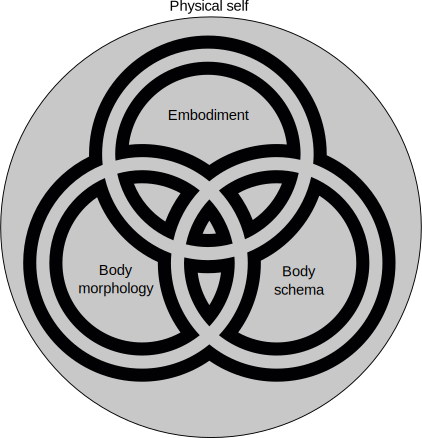
\includegraphics[width=0.5\textwidth]{overlapping_concepts}
		\caption{\textbf{Overlapping concepts.} Embodiment, body morphology, and body schema are three intersection concepts all involved in the definition of the physical self.}
		\label{fig:overlapping_concepts}
	\end{center}
\end{figure}
% ---



% SUBSECTION ================================================================================
\subsection{The body morphology}
The robot body morphology encompasses its physical structure, including the configuration of joints, limbs, sensors, and actuators \cite{Pfeifer2007SelfOrganizationEmbodiment}, playing a pivotal role in determining its capabilities and performance. The joints, serving as points of articulation, allow varied motion, with types like revolute, prismatic, and universal joints offering different degrees of flexibility. Limbs, the appendages extending from the body, consist of links and joints, defining the robot's range of motion and dexterity. Sensors provide information about the environment and internal state, influencing perception and decision-making. Actuators converting energy into mechanical motion and drive joint and limb movement, determining strength and endurance.

Design considerations for robot morphology involve stability, ensuring the robot withstands external forces and maintains balance. Dexterity is crucial for precise movements, achieved through joint, limb, and gripper design. Efficiency minimizes energy consumption for optimal performance, which is vital for autonomous or remote operation. Adaptability allows the robot to meet diverse task requirements or environmental conditions through modular designs or reconfigurable structures. Safety considerations prioritize minimizing risks to the robot and humans around it, incorporating protective tactile elements and elastic joints. Overall, a well-designed robot morphology integrates these key aspects and considerations to enhance its functionality and applicability.

The body morphology of a robot significantly influences its functionality and adaptability. Research in the field of robotics has emphasized the importance of the robot's body in achieving stable locomotion, efficient control, and adaptation to environmental challenges. For instance, the design and control of soft robots have focused on exploiting dynamics and morphology, such as the shape and length of the body and feet, to achieve stable walking \cite{Pfeifer2007SelfOrganizationEmbodiment}. Additionally, studies have shown that morphological variations can be a powerful technique for achieving resilient robots \cite{Pagliuca2020dynamicbodybrain}. Furthermore, it has been hypothesized that the morphological complexity of a robot should scale in relation to the complexity of its task environment \cite{Auerbach2012RelationshipEnvironmentalMechanical}.

In summary, the body morphology of a robot plays a crucial role in its locomotion, adaptability, and task-specific functionality. The research in this field underscores the importance of considering the dynamic interaction between a robot's body and its environment and the potential for co-optimizing morphology and control to enhance the robot's overall performance.

% SUBSECTION ================================================================================
\subsection{The body schema}

\subsubsection{General intuition}
The human body relies on a sophisticated neural representation known as the \textit{body schema} to navigate and interact with the surrounding environment, playing a foundational role in shaping the human experience of the physical self and the external world. This dynamic internal map within the brain encodes a multitude of attributes, ensuring the ability to perceive, move, and coordinate the body effectively.

The concept of the body schema has been defined in various ways in the scientific literature. One common definition is that it consists of sensorimotor representations guiding actions \cite{Maravita2003MultisensoryIntegrationBody}. Another widely accepted definition emphasizes the requirement for internal representations of the body's current posture and spatial extension \cite{Vignemont2010Bodyschemabody}. Fundamental to the body schema is the representation of the size and shape of different body parts, allowing for precise and coordinated movements. The brain's ability to accurately map the dimensions of the body contributes to the fluidity of human motion. Additionally, the body schema has been described as a means of obtaining information regarding body position in space from tactile, proprioceptive, visual, and other sensory modalities \cite{Medina2010mapsformspace}. %Sensations related to touch, pressure, temperature, and pain are seamlessly integrated into the body schema, enabling the perception and appropriate response to stimuli from the external environment. The tactile aspect of the body schema contributes to our ability to explore and understand the world through the sense of touch. 
These definitions illustrate the multifaceted nature of the body schema, encompassing sensorimotor guidance, spatial representation, and the integration of multisensory information.

%The body schema, as a dynamic internal representation, encompasses critical properties that shape the perception of the body and environment. Key features include spatial awareness, providing a continuous sense of body position and orientation. Proprioception allows for the perception of limb positions without visual cues, while motor programs facilitate purposeful movements. Multisensory integration combines information from vision, touch, and proprioception. Adaptability and plasticity enable adjustments through experience and learning. Joint angles and range of motion are crucial for coordinated movement. The incorporation of environmental cues allows responsive and context-specific actions. This multifaceted interplay of properties enables the body schema to play a central role in orchestrating seamless and adaptive interactions with the self and surroundings \cite{Vignemont20213C1Whatisbody,Morasso2015Revisitingbodyschema}.

The body schema, a complex and dynamic representation, plays a fundamental role in facilitating our effective interaction with the world. This intricate construct incorporates various properties crucial for our sensory and motor experiences. Spatial properties, encompassing the position, posture, overall shape, and size of individual body parts, as well as the body's relationship to gravity and the environment, form the foundation of the body schema. Kinesthetic properties involve the sensations of movement, touch, generated muscle force, and the resistance encountered during interactions. Vestibular properties contribute to our sense of balance, orientation in space, and awareness of the body's movement through space. Somatosensory properties, including the perception of temperature, pain, and pressure, as well as awareness of the body's surface and internal organs, further enrich the body schema. Additionally, the representation of mass, inertia, muscle forces, object properties, environmental properties, body ownership, and body boundaries collectively shape this intricate representation. Adaptability and plasticity enable adjustments through experience and learning. By integrating these diverse elements, the body schema enables humans to navigate their surroundings, interact with objects, and maintain a coherent sense of self in dynamic environments \cite{Vignemont20213C1Whatisbody,Morasso2015Revisitingbodyschema,Asada2018168Proprioceptionbodyschema}.


\subsubsection{The robot body schema}
Generally, the notion of body schema comprises sensorimotor representations of the body used to guide movement and action. For robotics this is, however, a far too general definition and incites the the question: \textit{what concretely is the body schema in robotics?}. From the various takes on this topic, efforts to consolidate an answer to this baffling question were provided in the comprehensive work by Hoffmann et al. \cite{Hoffmann2010Bodyschemarobotics}. Relevant to this dissertation is the discussion that the authors provide on explicit, articulated, and implicit models of the body schema. The first two categories pertain models where there is a direct correspondence between the body parts of
the robot and their representation in the sensors use to instantiate them measure variables associated to properties of the physical body. The main difference being that articulated models \cite{Grush2004emulationtheoryrepresentation} emphasize that the signals ought to come from embodied sensors. This latter property is referred as subjective or situated body schema by \cite{Hersch2008Onlinelearningbody}. The third category, implicit body schema, is more inline with traditional model learning methods in robotics and is aimed at constructing sensorimotor mappings.

%Although the authors reluctantly consider the explicit and objective body representations derived from model-based robotics are called  as they attempt to express the physical reality of the robot. More recently in \cite{Neemeh2021Bodyschemaautonomous}

As accentuated by the rich literature in model-based robotics, models of robots are required to achieve fine control and perform complex tasks. These models should include as much information as possible, explicit or implicit, of their body morphology (its embodiment). Most of the efforts associated with learning the body schema agree on the argument that an embodied robotic agent must autonomously learn and refine its body schema mainly proprioceptive information \cite{Morasso2015Revisitingbodyschema, Hoffmann2010Bodyschemarobotics}. Most the focus on calibration of a known kinematic structure \redtext{REF} with only few addressing the discovery of the body topology \redtext{REF}. \redtext{It is worth mentioning that there is no solid consensus in the literature about whether the body schema includes the inertial description of the parts composing the body. Yet, given that the body schema is used for planning and executing movements and that the sensation of effort (force and torque) is part of proprioception, it seems reasonable to assume the body schema must include such a representation.} Therefore, the question remains of what constitutes a body schema in robotics. %In this work we will bring back the discussion to the model-based robotics real and pair it with the understanding of the articulated model

To continue the discussion in this work the following conceptual definition of the robot body schema will be used:

\begin{definition}\label{def:robot_body_schema}
	%	The robot body schema is a representation of its body morphology that is mainly built from proprioceptive information. This representation includes the arrangement, geometry, and inertial properties of its parts and grants the ability to perceive the relative positions of limbs, and plan and execute movements without relying on visual cues. Adaptive and self-acquired, the robot body schema is a fundamental part of forward and inverse models used to plan and predict sensorimotor interactions beyond proprioception.
	The robot body schema is a representation of its body morphology primarily constructed from proprioceptive information. This representation encompasses the arrangement, geometry, and inertial properties of its parts, providing the capacity to perceive the relative positions of limbs and to plan and execute movements without relying on visual cues. Adaptive and self-acquired, the robot body schema plays a fundamental role in forward and inverse models, aiding in the planning and prediction of sensorimotor interactions beyond proprioception.
\end{definition}

%Ultimately, heightened spatial awareness is a product of the body schema, facilitating navigation and interaction with the environment. This attribute enables agents to move through space with precision, avoiding obstacles and adapting to changing surroundings, serving as a dynamic guide that shapes spatial understanding and enhances the ability to navigate the world.

%\subsubsection{Properties}
%The most important properties of the body schema include:
%
%1. Representation of the body's spatial properties: This encompasses the length of limbs and limb segments, their arrangement, the configuration of the segments in space, and the shape of the body surface.
%
%2. Integration of information from regions of the body and external space: The body schema is a set of fronto-parietal networks that integrate information originating from regions of the body and external space in a way that is functionally relevant to specific actions performed by different body parts.
%
%3. Short-term plasticity and reorganization: The body schema is characterized by short-term plasticity and reorganization, as demonstrated by the quick integration of tools into the body schema.
%
%4. Action-oriented overall coherence: It achieves an abstract or amodal representation while preserving an action-oriented overall coherence, allowing for the representation of the body for action.
%
%These properties highlight the dynamic and functional nature of the body schema, emphasizing its role in representing the body for action and its integration of spatial and sensory information from both the body and the external environment[1][3].
%
%Citations:
%[1] https://www.frontiersin.org/articles/10.3389/fnhum.2015.00083
%[2] https://academic.oup.com/book/41218/chapter-abstract/350687373?redirectedFrom=fulltext
%[3] https://www.ncbi.nlm.nih.gov/pmc/articles/PMC4330890/
%[4] https://psychology.fandom.com/wiki/Body_schema
%[5] https://academic.oup.com/book/41218/chapter/350687373
%The human body relies on an intricate neural representation known as the \emph{body schema} to navigate and interact with the surrounding environment. It plays a foundational role in shaping human experience of the physical self and the external world. This dynamic internal map within the brain encodes a multitude of attributes, ensuring our ability to perceive, move, and coordinate our bodies effectively.
%The concept of body schema has been defined in various ways in the scientific literature. One common definition is that the body schema consists of sensorimotor representations of the body that guide actions \cite{Maravita2003MultisensoryIntegrationBody}. Another widely accepted definition emphasizes the requirement for internal representation(s) of the body's current posture and spatial extension \cite{Vignemont2010Bodyschemabody}. Fundamental to the body schema is the representation of the size and shape of different body parts. This encoding allows for precise and coordinated movements. The brain's ability to accurately map the dimensions of the body contributes to the fluidity of human motion. . Additionally, the body schema has been described as a means of obtaining information regarding body position in space from tactile, proprioceptive, visual and other sensory modalities \cite{Medina2010mapsformspace}. Sensations related to touch, pressure, temperature, and pain are seamlessly integrated into the body schema. This incorporation allows for the perception and appropriate response to stimuli from the external environment. The tactile aspect of the body schema contributes to our ability to explore and understand the world through the sense of touch. These definitions highlight the multifaceted nature of the body schema, encompassing sensorimotor guidance, spatial representation, and the integration of multisensory information. An embodied robotic agent must autonomously learn and refine its body schema as a model representation of its morphology.The body schema is mainly built from proprioceptive information\cite{Morasso2015Revisitingbodyschema, Hoffmann2010Bodyschemarobotics}---as it grants us the ability to perceive the relative positions of our limbs without relying on visual cues--- and generally refers to an internal representation of the body, including the arrangement and geometry of its parts. Adaptive and self-acquired, the body schema is part of an agent's internal forward and inverse models and is used to plan and predict sensorimotor interactions. Ultimately, a heightened spatial awareness is a product of the body schema, facilitating navigation and interaction with the environment. This attribute enables agents to move through space with precision, avoiding obstacles and adapting to changing surroundings. The body schema serves as a dynamic guide, shaping spatial understanding and enhancing the ability to navigate the world.
% The body schema encodes information about joint angles and movements, providing the foundation for precise motor control.


\subsection{Embodiment}

%In the field of robotics, embodiment refers to the concept of how a robot's physical form and sensory-motor capabilities influence its interaction with the environment, shaping its perception and actions within its surroundings\cite{Duffy2000Intelligentrobotsquestion}. It involves the robot's physical structure, its situatedness, and its morphology, and how these factors go beyond mere functionality to impact human-robot interaction \cite{Miller2018EmbodimentSituatednessMorphology}. 

%In the realm of robotics, it represents a pivotal concept that transcends the mere mechanics of machinery. It encapsulates the profound idea of providing robots with a physical form and seamlessly intertwining this form with their sensory and motor capabilities. The essence of embodiment lies in acknowledging the significance of a robot's body, understanding its role in shaping interactions with the external world.
%Moreover, embodiment is evident in the way robots interact with their environment. Unlike purely computational models, embodied robots engage physically with their surroundings. They manipulate objects, traverse spaces, and respond directly to stimuli. This tangible interaction emphasizes the connection between a robot's physical presence and its functionality.

%At the heart of embodiment lies the concept of the body schema ----the robot's internal representation of its body and its relationship to the external world. This intricate awareness includes the robot's posture, position, and movement capabilities. The body schema is instrumental in achieving effective sensorimotor control and spatial awareness, essential for navigating and interacting in complex environments.


Embodiment, rooted in the notion that intelligence necessitates a body \cite{Pfeifer2006Howbodyshapes}, is a key concept in robotics. In this context, it refers to how a robot's physical form and sensory-motor capabilities shape its interactions within its environment, influencing perception and actions \cite{Duffy2000Intelligentrobotsquestion}. This involves considerations of the robot's physical structure, situatedness, and morphology, extending beyond functionality to impact interactions with the external world \cite{Miller2018EmbodimentSituatednessMorphology}.

At the core of embodiment is the physical form and morphology of a robot, including joints, limbs, sensors, and actuators. Beyond aesthetics, the design of a robot's physical form significantly influences movement, interaction capabilities, and overall functionality \cite{Pfeifer2006MorphologicalComputationConnecting}. Engineers delve into nuances of body morphology to tailor robots for specific tasks, whether exploration or assembly line operations.

Embodying robots goes beyond external structure, emphasizing that artificial agents have physical bodies interacting with the environment through seamless sensorimotor integration \cite{Lara2018EmbodiedCognitiveRobotics}. Sensors act as receptors conveying information, and actuators enable the robot to act upon sensory input, resulting in adaptive behavior \cite{Pfeifer2007SelfOrganizationEmbodiment,Der2014RoleEmbodimentSelf}. This sensorimotor integration distinguishes embodied robotics from abstract computational systems.

Embodiment also involves situatedness, where robots directly interact with their environment, enhancing autonomy and adaptability \cite{Brooks1991NewApproachesRobotics}. Incorporating action and sensory-motor experiences as sources of statistical regularities is crucial for cognitive robots \cite{Pezzulo2013ComputationalGroundedCognition}.

The concept of body schema, closely linked to embodiment, represents an internal model encompassing a robot's body arrangement, geometry, and movements. It serves as a dynamic tool for spatial awareness. Adaptability is a hallmark of embodied robots, stemming from the close coupling of their physical bodies and control systems, enabling dynamic responses to environmental changes.

In essence, embodiment in robotics transcends traditional boundaries, transforming robots into physically present, interactive agents. The intricate dance between physical form, sensorimotor integration, body schema, and adaptability enriches robotics, fostering the development of sophisticated, versatile, and context-aware systems.

%Embodiment is associated to the idea that intelligence requires a body \cite{Pfeifer2006Howbodyshapes}. In the field of robotics, embodiment refers to the concept of how a robot's physical form and sensory-motor capabilities influence its interaction with the environment, shaping its perception and actions within its surroundings\cite{Duffy2000Intelligentrobotsquestion}. It involves the robot's physical structure, its situatedness, and its morphology, and how these factors go beyond mere functionality shaping the interactions with the external world. \cite{Miller2018EmbodimentSituatednessMorphology}. 
%
%Central to the concept of embodiment is the physical form and morphology of a robot. This encompasses the intricate arrangement of joints, limbs, sensors, and actuators---the very components that define a robot's structure. The design of a robot's physical form goes beyond aesthetics; it fundamentally influences its movement, interaction capabilities, and overall functionality \cite{Pfeifer2006MorphologicalComputationConnecting}. Engineers and researchers delve into the nuances of body morphology to create robots tailored for specific tasks, whether exploration, assembly line operations, or other applications.
%
%Embodying robots extends beyond their external structure; it involves  the idea that artificial agents have physical bodies and interact with their environment through the seamless integration of sensorimotor capabilities \cite{Lara2018EmbodiedCognitiveRobotics}. Sensors are the robot's sensory receptors that convey information about itself and its environment. Actuators are the means through which the robot acts upon this sensory input. The synthesis of sensing and acting results in adaptive behavior \cite{Pfeifer2007SelfOrganizationEmbodiment,Der2014RoleEmbodimentSelf}, allowing the robot to respond dynamically to environmental stimuli. This sensorimotor integration is a hallmark of embodied robotics, distinguishing it from abstract computational or simulation-based systems.
%
%Embodiment in robotics also encompasses the idea of situatedness, where robots are situated in the world and interact directly with their environment, influencing their behavior \cite{Brooks1991NewApproachesRobotics}. This direct interaction with the environment allows robots to experience the world and carry out tasks in unstructured environments, contributing to their autonomy and adaptability. Additionally, embodiment in robotics involves the incorporation of action and sensory-motor experiences as sources of statistical regularities that are learned and utilized by cognitive robots \cite{Pezzulo2013ComputationalGroundedCognition}.
%
%The concept of body schema is closely intertwined with embodiment in robotics, representing an internal model within a robot encompassing its body's arrangement, geometry, and movements. It serves as a dynamic and adaptive tool for the robot's awareness of its physical structure and spatial orientation. Embodiment, a broader concept, involves providing a robot with a physical form and integrating it with sensory and motor capabilities, emphasizing tangible interaction with the physical world. The relationship lies in the body schema's role as a crucial component of embodied robotics, serving as an internal map guiding the robot's movements and interactions, bridging the gap between its physicality and sensorimotor control systems. The body schema facilitates effective navigation, spatial awareness, and adaptability, contributing significantly to the embodiment process, where the robot embodies its presence through dynamic interactions in the external environment.
%
%Adaptability is another hallmark of embodied robots. Their movements and responses are not rigidly pre-programmed but are rather flexible and dynamic. This adaptability stems from the close coupling of a robot's physical body and its control systems. It allows robots to adjust their behavior based on changes in the environment, unexpected obstacles, or evolving task requirements.
%
%In essence, embodiment in robotics transcends the traditional boundaries of machinery and computation. It transforms robots from abstract entities into physically present, interactive agents. The intricate dance between the robot's physical form, sensorimotor integration, body schema, and adaptability enriches the field of robotics, opening avenues for the development of more sophisticated, versatile, and context-aware robotic systems.



\subsubsection{Embodiment and information structure}
\TODO
According to \cite{LungarellaEmbodimentInformationCausal}






% ---
\begin{figure}
	\begin{center}
		\includegraphics[width=0.7\textwidth]{implications_of_embodiment}
		\caption{\textbf{Implications of embodiment.} From Pfeifer et al. \cite{Pfeifer2007SelfOrganizationEmbodiment}. Reprinted with permission from AAAS.}
	\end{center}
\end{figure}
% ---


\begin{center}
	\begin{tabular}{ |m{0.3\textwidth}|m{0.35\textwidth}|m{0.35\textwidth}| } 
		\hline
		\textbf{Concept} & \textbf{Definition} & \textbf{Relationship} \\ 
		\hline
		Physical self & Our awareness of our own body and its interactions with the environment & Foundation of embodiment \\ 
		\hline
		Embodiment & The idea that our thoughts, feelings, and experiences are shaped by our physical bodies & Dynamic representation of body's physical structure and position in space \\ 
		\hline
		Body schema	 & Our internal model of our body's physical structure and its position in space & Manifestation of embodiment \\ 
		\hline		
		Body morphology & The physical structure of our body, including its size, shape, and proportions & Influences embodiment and the physical self
	\end{tabular}
\end{center}
% ===========================================================================================
%                                           |                                               |
% -------------------------------------- SECTION -------------------------------------------|
%                                           |                                               |
% ===========================================================================================
\section{Robot equations of motion}
\subsection{Forward and inverse dynamics}
\subsection{The Newton-Euler formulation of the inverse dynamics}

Extension for floating base robots with flexible joints and links have been presented elsewhere \cite{Khalil2017GeneralDynamicAlgorithm}
% The kinematics forward recursion
% The dynamics backward recursion
\subsection{Composition of the kinematics and dynamics}
%bsection{Basics of robot system identification}
%bsubsection{Kinematic calibration}
%bsubsection{Inertial parameter identification}
% For fixed based robots
% For floating base robots

% ===========================================================================================
%                                           |                                               |
% -------------------------------------- SECTION -------------------------------------------|
%                                           |                                               |
% ===========================================================================================
\section{Robot proprioception}
\TODO Paraphrase and reference this section. Use this \cite{Asada2018168Proprioceptionbodyschema}

Proprioception is required to ensure the plasticity of the body schema \cite{Cardinali2016Proprioceptionisnecessary}

\subsection{The role of proprioception}

Much of
this knowledge about position and movement of the limbs
and trunk is provided by sensations arising in propriocep-
tors. The information they provide allows us to maneuver
our way around obstacles in the dark and be able to manip-
ulate objects out of view.

Traditionally, however, the term propri-
oceptor has been restricted to receptors concerned with
conscious sensations, and these include the senses of limb
position and movement, the sense of tension or force, the
sense of effort, and the sense of balance.

To motivate the importance of robot proprioception, this section first discusses the role it plays in living systems. This section relies on the material presented in 
As proprioceptive sensations, the senses of effort, force, and
heaviness are distinct in that they are always associated with
motor commands, while kinesthetic sensations can arise in a
passive limb. It implies that for the senses of force and heavi-
ness the peripheral input is always reafferent in origin. An-
other issue to consider is the meanings of the terms. What do
we mean by a sense of effort as distinct from a sense of tension?

 It is
concluded that a sense of effort, arising centrally in associ-
ation with motor commands, is able to contribute to a num-
ber of proprioceptive sensations including the sense of limb
position and the sense of limb movement.




\subsection{Definition}
\subsection{Human and robot proprioception}
\subsection{A sensor suite for robot proprioception}


\section{The body schema in robotics}

\subsection{Biological body schema}
The biological body schema refers to the internal representation that the brain maintains of the body's spatial configuration and the relationship between its parts. It is a dynamic and flexible neural map that integrates sensory information, motor commands, and past experiences to create a coherent and updated perception of one's own body. The body schema plays a crucial role in motor control, spatial awareness, and the ability to interact effectively with the environment.

Key elements of the biological body schema include proprioception (awareness of the body's position in space), tactile sensations, and motor control. Proprioceptors, which are sensory receptors in muscles, tendons, and joints, provide information about the body's position and movement. This information is continuously processed by the brain to maintain an accurate and up-to-date representation of the body.

The biological body schema is not static; it can be modified through experiences, learning, and adaptation. It is essential for various cognitive functions, including spatial orientation, hand-eye coordination, and the execution of complex motor tasks. Disruptions to the body schema, such as neurological disorders or injuries, can lead to difficulties in motor control and spatial perception. Understanding the biological body schema is crucial in fields like neuroscience, psychology, and rehabilitation, as it provides insights into how the brain perceives and interacts with the body and the external environment.


\subsection{Body features encoded in the body schema}
The body schema representation in the brain encodes various attributes of the body to facilitate perception and interaction with the environment. These attributes include:

\paragraph*{Body Size and Shape} The brain has a representation of the size and shape of different body parts. This allows for accurate and coordinated movements and interactions.

2. **Body Position:** The body schema includes information about the spatial orientation and position of body parts in relation to each other. This is essential for coordinating movements and maintaining balance.

3. **Proprioception:** This is the sense of the relative position of one's own body parts and the effort being employed in movement. Proprioceptive information helps in knowing the positions of limbs without having to visually observe them.

4. **Joint Angles:** The body schema encodes information about the angles and movements of joints, allowing for smooth and coordinated motor control.

5. **Touch and Tactile Sensations:** Sensations related to touch, pressure, temperature, and pain are integrated into the body schema. This information helps in perceiving and responding to stimuli from the external environment.

6. **Spatial Awareness:** The body schema contributes to spatial awareness, allowing individuals to navigate and interact with the surrounding space effectively.

7. **Body Image:** While related, body image is a more complex concept that involves cognitive and emotional aspects of how an individual perceives their own body. The body schema contributes to this perception but is not the sole factor.

8. **Motor Programs:** The body schema is closely tied to motor control and the execution of movement. It helps in generating and executing motor programs for voluntary actions.

These attributes collectively contribute to a coherent and dynamic representation of the body, enabling individuals to interact with their environment in a purposeful and adaptive manner. The body schema is not fixed but can be modified based on experiences, learning, and changes in the body itself.



\subsection{Some context}
\redtext{\say{The body schema is viewed as a set of fronto-parietal networks that integrate information originating from regions of the body and external space in a way that is functionally relevant to specific actions performed by different body parts$\ldots$ It represents the body's spatial properties, including the length of limbs and limb segments, their arrangement, the configuration of the segments in space, and the shape of the body surface$\ldots$ The body schema is characterized by short-term plasticity and reorganization, as shown by the quick integration of tools into the body schema}} \cite{Morasso2015Revisitingbodyschema}

\say{The concept of body schema is related to model learning in robotics as it provides a framework for robots to understand and represent their own bodies and the surrounding environment. Research in this area aims to enable robots to improve their capabilities by automatically synthesizing, extending, or adapting a model of their body, similar to how the human body schema allows for adaptive and coordinated movement. This involves integrating information from multiple sensory modalities and controlling complex bodies, which are desirable capabilities for robots. By studying the body representations in biology from a functional or computational perspective, researchers seek to develop robotic systems that can effectively model their own bodies and interact with the environment in a more human-like manner. Therefore, the concept of body schema plays a crucial role in the development of robotic systems that can learn and adapt to their own physical characteristics and the surrounding world.}


The concept of body schema and its relevance to model learning in robotics is well-supported in the scientific literature. While there are no specific sources directly linking the concept of body schema to model learning in robotics, the following sources provide relevant information about the body schema and its implications:

(1) The article "Influence of the Body Schema on Multisensory Integration: Evidence from the Mirror Box Illusion" in Scientific Reports - Nature discusses the influence of the body schema on multisensory integration, which is a fundamental aspect of robotic model learning.

(2) The paper "Neuroplasticity in the blind and sensory substitution for vision" on ResearchGate explores neuroplasticity in the blind, which is relevant to understanding how the body schema is developed and adapted in the absence of vision, a concept that can be applied to robotics.

(3) The article "Does visual experience influence arm proprioception and its lateralization? Evidence from passive matching performance in congenitally-blind and sighted adults" in ScienceDirect provides insights into the relationship between visual experience and proprioception, which is foundational to the development of the body schema and has implications for robotics.

(4) The study "Degraded vision affects mental representations of the body" published on Taylor \& Francis Online discusses the impact of degraded vision on mental representations of the body, including the shift from a pictorial representation of the body to a somatosensory one, which is relevant to understanding the body schema in the context of robotic model learning.

While these sources do not directly address the application of body schema to model learning in robotics, they provide valuable insights into the development and influence of the body schema, which can be extrapolated to understand its potential relevance to model learning in robotics.

%Citations:
%[1] https://www.nature.com/articles/s41598-017-04797-0
%[2] https://www.researchgate.net/publication/262840022_Neuroplasticity_in_the_blind_and_sensory_substitution_for_vision
%[3] https://www.sciencedirect.com/science/article/abs/pii/S030439402300294X
%[4] https://www.tandfonline.com/doi/full/10.1080/13506285.2023.2186997

% ===========================================================================================
%                                           |                                               |
% -------------------------------------- SECTION -------------------------------------------|
%                                           |                                               |
% ===========================================================================================
\section{Driving online learning: Gradient descent}
\begin{figure}[h!]
	\begin{center}
		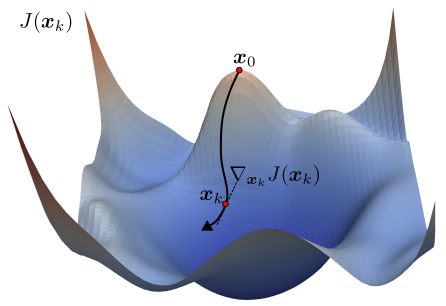
\includegraphics[width=0.5\textwidth]{gradient_descent_concept.pdf}
	\end{center}
	\caption{Concept art gradient descent. Image credits: \url{https://www.cs.umd.edu/~tomg/projects/landscapes/}}
\end{figure}
\subsection{Offline and online learning}
In the realm of machine learning, online learning and offline learning represent distinct approaches to model training. Online learning, or incremental learning, involves learning the model as new data becomes available, typically processing one observation at a time. In this scenario, the learning algorithm's parameters are updated after each individual training instance, making it particularly advantageous for systems dealing with a continuous flow of data that must rapidly adapt to changing conditions. On the other hand, offline learning, also known as batch learning, entails training the model over all observations in a dataset $\mathcal{D}$ simultaneously. The model is trained with a static dataset, and the parameters are updated once the learning process is complete for the entire dataset. %Offline learning is more prevalent in industry due to its various advantages, such as simplicity and ease of implementation. In essence, online learning is a dynamic approach where the model adapts to new data in real-time, while offline learning is a more static method where the model is trained on a fixed dataset.

%In contrast, online learning excels in real-time adaptation and efficient resource utilization, making it more appropriate for scenarios with continuously changing data patterns[4][12]. 

\subsection{Fundamentals of gradient descent}
Gradient descent (GD) is in essence an optimization algorithm to sequentially minimize a \emph{cost function} $J(\bm{x})$ with respect to a given set of parameters $\bm{x} \in \mathbb{R}^d$ moving in the direction opposite to its gradient $\nabla_{\bm{x}}J(\bm{x})$ at the current point $\bm{x}_k$. GD is considered a local optimizer as it primarily finds a local minimum of $J$. The algorithm can be summarized in a iterative process expressed in the simple equation
% ---
\begin{equation}\label{eq:gradient_descent}
	\bm{x}_{k+1} = \bm{x}_k - \eta  \nabla_{\bm{x}_k} J(\bm{x}_k;\mathcal{D}),
\end{equation}  
% ---
which gives the update $\bm{x}_{k+1}$ to the optimization variables using a \emph{learning rate} $\eta$ that controls the size of the step given in the negative direction of the gradient. If this hyperparameter is too small, the updates $\bm{x}_{k+1}$ will differ slightly from $\bm{x}_k$ and convergence will take a long time. On the contrary, if $\eta$ is too large, the parameter updates may oscillate around a local optima and even diverge. 

From the number of data points from an already-collected dataset $\mathcal{D}$ that are used to represent the optimization cost function $J$, three variants of GD are typical: batch, stochastic, and mini-batch GD. If all data in $\mathcal{D}$ is used to compute the gradient, it is called batch GD. It relies on a static dataset and substantial computational resources (CPU, memory, and storage) for training and thus lacks the flexibility to adapt incrementally to new data. This inability to incorporate new observations in real-time hinders its applicability for online learning in dynamic environments with constantly evolving data streams. 
%The time-intensive nature of batch GD exacerbates its limitations, as updating the model with new data requires the retraining of the entire dataset, proving computationally expensive. Additionally, batch GD is less flexible in handling changing or large datasets, making it more suitable for stable scenarios with ample resources. Finally, batch learning systems lack the ability to learn incrementally, a significant drawback when dealing with streaming data or scenarios where the data distribution frequently changes.

Stochastic Gradient Descent (SGD) \cite{Bottou2012Stochasticgradientdescent} serves as a simplification of batch GD and is widely employed machine in machine learning for online learning due to its efficiency with large-scale datasets and its ability to adapt to new data one observation at a time. Its advantages lie in its speed, processing quicker parameter updates, and memory efficiency. A recent review \cite{Tian2023RecentAdvancesStochastic} discusses the the properties of SGD as a standard optimization algorithm in deep learning. Despite its ability to escape local minima, the noisy updates of SGD and bouncing behavior near the minimum can yield good but non-optimal solutions \redtext{REF}. When the gradient of the cost function is computed using a small subset or mini-batch of $\mathcal{D}$, rather than a single example or the entire dataset, SGD becomes mini-batch GD. This approach reduces the noise in the parameter updates compared to SGD, leading to more stable convergence. It allows for computational efficiency as the mini-batch can be processed in parallel, and it is typically faster than batch GD for convergence.

\subsection{Improved gradient descent}
The challenges associated with standard (commonly named vanilla) GD encompass critical issues. First, there is the already mentioned sensitivity to the selected learning rate $\eta$. Noisy gradients are a particular problem of SGD and mini-batch GD. These may lead to slower and less stable training compared to batch GD. The algorithms may also encounter obstacles like local minima and saddle points, particularly problematic in non-convex optimization problems, hindering the discovery of the global minimum.

Various improvements have been proposed to improve vanilla GD in recent years \cite{Ruder2016overviewgradientdescent,Tian2023RecentAdvancesStochastic}. Noteworthy among these enhancements are the incorporation of a momentum term, adaptive learning rate mechanisms, and measures to handle very small step sizes. The momentum term, functioning as a moving average over past gradients, serves to smooth out steps in gradient descent, thereby mitigating oscillations and expediting convergence. Its purpose is to combat issues such as bouncing around the search space and getting stuck in flat regions, ultimately elevating the optimization algorithm's efficacy and yielding superior final results.

The adaptive learning rate, tailored individually for each parameter based on the square root of the sum of the squares of historical gradients, facilitates larger updates for infrequent parameters and smaller updates for frequent ones. This adaptability proves beneficial for handling sparse data and managing sparse gradients. The approach aims to expedite convergence in the presence of sparse data by adjusting the learning rate according to the loss function's geometry. This allows for swift convergence in steep gradient directions and more cautious updates in flatter gradient directions.

However, a notable drawback of learning rate adaption is the its potential reduction to infinitesimally small values over time, limiting the ability to acquire additional knowledge. To counteract this issue, a decaying average of squared gradients was proposed to adjust the step size for each parameter. This adaptive strategy stabilizes the learning process, preventing oscillations in the optimization trajectory and proving effective for non-convex optimization problems commonly encountered in machine learning.

%
%\paragraph*{ Gradient descent with momentum.} In cost functions that change rapidly in one parameter direction and rather slowly in others, regular GD oscillates heavily in directions quasi perpendicular to the gradient and makes meager progress towards the minimum. This algorithm dampens this oscillations and accelerateseAlso known as Nesterov's accelerated gradient, Accelerates faster towards the minimum and increases the chance of escaping local minima
%\subsection{Adaptive gradient descent}
%Known commonly as AdaGrad. It adapts the updates relative to the sum of the accumulated squared gradients. This has the effect of balancing the increments given to all descent directions and results in a \say{straighter} path towards the minimum. Unfortunately, because of the gradient accumulations, updates quickly become rather small and this leads to a rather slow convergence,
%
%\subsection{RMSProp}
%Root Mean Square Propagation. It adds decay rate to the sum of past squared gradient giving important to only the recent ones.n
%
%
%\begin{center}
%	\begin{tabular}{ |c|c|c| } 
%		\hline
%		\textbf{Algorithm} & \textbf{Update} & \textbf{Details} \\ 
%		\hline
%		Momentum & cell5 & cell6 \\ 
%		\hline
%		NAG & cell8 & cell9 \\ 
%		\hline
%		Adagrad & cell8 & cell9 \\ 
%		\hline		
%		Adadelta & cell8 & cell9 \\ 
%		\hline
%		RMSProp & cell8 & cell9 \\ 
%		\hline
%		ADAM & cell8 & cell9 \\ 
%		\hline
%		AdaMax & cell8 & cell9 \\ 
%		\hline
%		NADAM & cell8 & cell9 \\ 
%		\hline
%		NADAM & cell8 & cell9 \\ 
%\hline		
%	\end{tabular}
%\end{center}



\subsubsection{Adaptive moment estimation: Adam}
Adaptive Moment Estimation GD, commonly known as Adam \cite{Kingma2014Adammethodstochastic}, has become a powerful optimization technique standard in machine learning. Adam is an adaptive learning algorithm that refines SGD approach by incorporating both first-order moment estimates ($m_t$) and second-order moment estimates ($v_t$) of the gradients; that is
% ---
\begin{align}\label{eq:adam_mean_and_uncentered_variance}
	\begin{split} 
		m_k &= \beta_1 m_{k-1} + \left(1 - \beta_1 \right) \nabla_{\bm{x}_k} J(\bm{x}_k;\mathcal{D}) \\ 
		v_k &= \beta_2 v_{k-1} + \left(1 - \beta_2\right) \left( \nabla_{\bm{x}_k} J(\bm{x}_k;\mathcal{D}) \right)^2 ,
	\end{split}
\end{align}
% ---
where the moving averages of the momentum term and the squared gradients  is adjusted via the discount factors $\beta_1 \in [0,1]$ and $\beta_2 \in [0,1]$. The adaptive nature of Adam stems from dynamically adjusting learning rates $\left\lbrace \eta_i\right\rbrace^d_{i=1}$ for each parameter based on the historical gradient information. This feature addresses a longstanding challenge in machine learning---manual tuning of learning rate $\eta$. The ability of Adam to autonomously adjust rates during training alleviates the need for meticulous parameter tuning, a characteristic that sets it apart from its predecessors.

A fundamental strength of Adam lies in its incorporation of momentum, which enables Adam to persist in the correct direction, surmounting obstacles such as flat regions or saddle points in the cost function $J$. Furthermore, Adam introduces a bias correction mechanism, particularly beneficial in the initial stages of training when moment estimates might be imprecise\footnote{The terms $v_k$ and $m_k$ are biased towards their zero initial value.}. This correction, computed as
% ---
\begin{align}\label{eq:adam_bias_correction}
	\begin{split} 
		\hat{m}_k &= \dfrac{m_k}{1 - \beta_1} \\ 
		\hat{v}_k &= \dfrac{v_k}{1 - \beta_2},
	\end{split} 
\end{align}
% --
enhances the accuracy of the mean and uncentered variance estimates in \eqref{eq:adam_mean_and_uncentered_variance}, contributing to the algorithm's robustness. The update rule for Adam, based on Eqs.~\eqref{eq:adam_bias_correction} and \eqref{eq:adam_mean_and_uncentered_variance}, yields
% ---
\begin{equation}
	x_{k+1} = x_{k} - \dfrac{\eta}{\sqrt{\hat{v}_t} + \epsilon} \hat{m}_t.
\end{equation}
% ---
Note that according to \cite{Kingma2014Adammethodstochastic}, the default values of $\beta_1 = 0.9$, $ \beta_2 = 0.999 $, and $\epsilon =10^{-8}$ seem to work well in practice.

Adam's computational efficiency is a standout feature, showcasing its prowess in a diverse array of applications. It has demonstrated a tendency to converge faster and demand less hyperparameter tuning than traditional SGD. Notably, Adam's adaptability to sparse or high-dimensional data renders it well-suited for complex models where different parameters may necessitate varying learning rates. This adaptability is particularly advantageous in real-world scenarios where data is inherently noisy.

The algorithm's ability to handle noisy gradients effectively speaks to its stability during training, contributing to the robustness that makes Adam a preferred choice in modern machine learning applications.% While Adam's success is undeniable, it is essential to acknowledge that the choice of optimization algorithm depends on specific problem characteristics. Variants such as RMSprop or AdaGrad may also prove effective in certain contexts, and the performance can vary based on the dataset and the model architecture.


%\paragraph*{ Gradient descent with momentum.} In cost functions that change rapidly in one parameter direction and rather slowly in others, regular GD oscillates heavily in directions quasi perpendicular to the gradient and makes meager progress towards the minimum. This algorithm dampens this oscillations and accelerateseAlso known as Nesterov's accelerated gradient, Accelerates faster towards the minimum and increases the chance of escaping local minima
%\subsection{Adaptive gradient descent}
%Known commonly as AdaGrad. It adapts the updates relative to the sum of the accumulated squared gradients. This has the effect of balancing the increments given to all descent directions and results in a \say{straighter} path towards the minimum. Unfortunately, because of the gradient accumulations, updates quickly become rather small and this leads to a rather slow convergence,
%
%\subsection{RMSProp}
%Root Mean Square Propagation. It adds decay rate to the sum of past squared gradient giving important to only the recent ones.n
%
%\subsection{ADAM gradient descent}
%Adaptive Moment Estimation. In essence a combination between the effects of momentum and RMSProp; that is, it inherits the speed from momentum and the ability to adapt the gradient directions.
\subsubsection{AMS gradient descent}


AMSGrad is a gradient descent method that aims at convergence issues faced by Adam and its variations \cite{Reddi2019convergenceadam}; which have been observed to exhibit issues related to the learning rate, where it may become too aggressive and lead to poor convergence behavior in certain scenarios. AMSGrad tries to address this issue by modifying the way it updates the parameters. 

The key improvement introduced by AMSGrad lies in its handling of the adaptive learning rates for each parameter. In the original Adam algorithm, the learning rates are adapted based on the exponential moving averages of the first-order moment (mean) and the second-order moment (uncentered variance) of the gradients. However, Adam does not incorporate a mechanism to correct the bias in the estimate of the second-order moment, which can lead to an overly aggressive decrease in the learning rates.

AMSGrad addresses this limitation by modifying the update rule for the moving average of the second-order moment. Unlike Adam, AMSGrad maintains a running average of the past squared gradients for each parameter without bias correction. Particularly, instead of using $\hat{v}_t$ as in \eqref{eq:adam_bias_correction}, its previous value $\hat{v}_{k-1}$ is used as long as it is greater than the current value computed according to \eqref{eq:adam_mean_and_uncentered_variance}; i.e.,
% ---
\begin{equation}
	\hat{v}_t = \text{max}(\hat{v}_{t-1}, v_t).
\end{equation}
% ---
The update rule for AMSGrad 
% ---
\begin{equation}
	x_{k+1} = x_{k} - \dfrac{\eta}{\sqrt{\hat{v}_t} + \epsilon} m_t
\end{equation}
% ---
excludes also the regularization of the first momentum term. The alteration to the second moment ensures that the denominator in the learning rate calculation does not become excessively small over time, preventing the learning rate from growing uncontrollably small.

In essence, AMSGrad aims to provide a more stable and consistent learning rate, preventing scenarios where the learning rate diminishes rapidly and adversely affects convergence. By addressing this issue, AMSGrad aims to offer improved convergence behavior and generalization, particularly in cases where Adam might exhibit erratic behavior due to the uncorrected bias in the second-order moment estimate.


% ===========================================================================================
%                                           |                                               |
% -------------------------------------- SECTION -------------------------------------------|
%                                           |                                               |
% ===========================================================================================
\section{Fundamentals of graph theory}

\subsection{Definition of a graph}
A graph $\mathcal{G} = \left(\mathcal{V}, \mathcal{E}\right)$ is a mathematical construct the represents the interconnections between the elements of a system. These elements are represented as a set $ \mathcal{V}=\left\lbrace v_i\right\rbrace^n_{i=1}$ of $n$ \emph{nodes} (also called \emph{vertices}) and their connections are depicted as a set of \emph{edges} $ \mathcal{E}= \left\lbrace e_i\right\rbrace^m_{i=1} \subseteq \mathcal{V} \times \mathcal{V} $. Note that it is possible that an edge connects a node to itself, in which case the edge defines a self loop.
% ---
%\begin{figure}[th!]
%	\begin{center}
%		\includegraphics[width=0.5\textwidth]{example_graph.pdf}
%		\caption{Example graph.}
%		\label{fig:example_graph}
%	\end{center}
%\end{figure}
% ---
\begin{figure*}[!h]
	\centering	
	\hspace*{\fill}
	\begin{subfigure}[t]{0.32\textwidth}
		\subcaption{}
		\includegraphics[width=\textwidth]{example_graph.pdf}
		\label{fig:example_graph}
	\end{subfigure}	
	\hfill
	\begin{subfigure}[t]{0.32\textwidth}
		\subcaption{}
		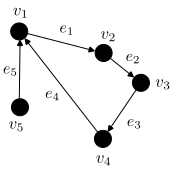
\includegraphics[width=\textwidth]{example_digraph.pdf}
		\label{fig:example_digraph}
	\end{subfigure}
	\hspace*{\fill}	
	\caption[] {\label{fig:graph_examples} \textbf{Two basic types of graphs}. (\subref{fig:example_graph}) An undirected and (\subref{fig:example_digraph}) a directed graph.}
\end{figure*}

%\begin{figure*}[!h]
%	\centering	
%	\hspace*{\fill}
%	\begin{subfigure}[t]{0.32\textwidth}
%		\subcaption{}
%		\includegraphics[width=\textwidth]{f6a_phantomx_hexapod.pdf}
%		\label{fig:phantomx_robot}
%	\end{subfigure}	
%	\hfill
%	\begin{subfigure}[t]{0.32\textwidth}
%		\subcaption{}
%		\includegraphics[width=\textwidth]{f6b_phantomx_pi_graph_kinematics.pdf}
%		\label{fig:phantomx_pigraph_kin_clusters}
%	\end{subfigure}
%	\hfill
%	\begin{subfigure}[t]{0.32\textwidth}
%		\subcaption{}
%		\includegraphics[width=\textwidth]{f6c_phantomx_morphology.pdf}
%		\label{fig:phantomx_morphology}
%	\end{subfigure}	
%	\hspace*{\fill}
%	\\
%	\hspace*{\fill}
%	\begin{subfigure}[t]{0.96\textwidth}
%		\subcaption{}
%		\includegraphics[width=\textwidth]{f6d_phantomx_morphology_errors_offline.pdf}
%		\label{fig:phantomx_morphology_errors_offline}
%	\end{subfigure}	
%	\hspace*{\fill}
%	\\
%	\hspace*{\fill}
%	\begin{subfigure}[t]{0.96\textwidth}
%		\subcaption{}
%		\includegraphics[width=\textwidth]{f6e_phantomx_morphology_errors_online.pdf} 		
%		\label{fig:phantomx_morphology_errors_online}
%	\end{subfigure}	
%	\hspace*{\fill}	
%	\caption[] {\label{fig:hexapod_simulated_results} \textbf{The hexapod robot}. (\subref{fig:phantomx_robot}) the PhantomX hexapod robot with its IMUs (red spheres), (\subref{fig:phantomx_pigraph_kin_clusters}) the kinematics graph $\mathcal{G}^{\mathcal{K}}_\pi$, (\subref{fig:phantomx_morphology}) the learned kinematic structure, errors in the estimated body structure via (\subref{fig:phantomx_morphology_errors_offline}) offline learning and (\subref{fig:phantomx_morphology_errors_online}) online learning (blue: difference rotation errors $\bar{\delta}~[\text{rad}]$, orange: sensor-to-sensor vector errors $\bar{\tilde{r}}~[\text{m}]$).}
%\end{figure*}
Two nodes $i$ and $j$ are said to be \emph{adjacent} if there is an edge $e$ connecting them. Similarly, the edge $e$ connecting the nodes is called \emph{incident} to $i$ and $j$. For example, the nodes $v_1$ and $v_4$ in Fig.~\ref{fig:example_graph} are adjacent to each other and the edge $e_4$ is incident to both nodes. The number of edges that are incident to a node is the \emph{degree} of the vertex. 

A \emph{path} represents a potential sequence of edges connecting any two given nodes. The number of edges determines the \emph{length} of the path. A graph is said to be \emph{connected} if there is at least one path between every pair of nodes; otherwise, it is labeled \emph{disconnected}. A \emph{cycle} constitutes a path comprising a minimum of three edges, where the initial and final vertices are identical, and no vertices are repeated in between. Lastly, a graph is \emph{complete} if there exists a path connecting every pair of nodes. Notice that the maximum number of edges in an undirected graph with $n$ nodes is $n(n-1)/2$

An \emph{undirected} graph lacks any specified direction assigned to its edges, meaning the connections between nodes are bidirectional. On the other hand, a \emph{directed} graph, commonly referred to as a \emph{digraph}, introduces directionality to its edges. In a directed graph, each edge has an explicit direction, indicating a one-way flow from one node to another. This directional information adds an extra layer of complexity to the relationships within the graph, as opposed to the bidirectional nature of edges in an undirected graph.

%A graph (or network) is a structure  that expresses the relationships between a set of vertices $ \mathcal{V}=\left\lbrace v_i\right\rbrace^m_{i=1}$ via a set of edges $ \mathcal{E}\subseteq \mathcal{V} \times \mathcal{V} $ with weights $ \bm{W}: \mathcal{V} \times \mathcal{V}\to \mathbb{R}_+$. Known as the weighted adjacency matrix, $ \bm{W} $ serves as the algebraic representation of $\mathcal{G}$.
A \emph{weighted} graph $ \mathcal{G}\big(\mathcal{V},\mathcal{E},\bm{W}\big) $ associates numerical value, a weight, to each edge. The weights with weights $ \bm{W}: \mathcal{V} \times \mathcal{V}\to \mathbb{R}_+$ express some quantitative measure such as distance, cost, time, or any other relevant metric depending on the context of the graph. Unlike an unweighted graph, where edges simply represent connections between nodes, a weighted graph provides additional information about the relationships between nodes. For a weighted graph, the \emph{strength} of a vertex corresponds to the sum of the edge weights associated with it.


\subsection{Algebraic representation of a graph}
A graph with $n$ vertices can be represented as a square $n\times n$ matrix $\bm{A}$. This algebraic representation is called the \emph{adjacency matrix} and depicts the graph's connectivity pattern; that is, the elements of the matrix indicate whether pairs of vertices $\left(i,j\right)$ are adjacent or not in the graph. Formally,
the elements of a \emph{binary} adjacency matrix $\bm{A}$ are determined as follows
% ---
\begin{equation}
	\left(\bm{A}\right)_{i,j} =
	\begin{cases}
		1 & \text{if and edge connects nodes $i$ and $j$}\\
		0 & \text{otherwise}.
	\end{cases}
\end{equation}
% --
By extension, a \emph{weighted} adjacency matrix $\bm{W}$ denotes a weighted connection for some of the $\left(i,j\right)$ entries, i.e $\left(\bm{W}\right)_{i,j} \in \mathbb{R}_+$. If the graph is undirected, the adjacency matrix is symmetric, which implies that $\bm{A}=\bm{A}^\intercal$ and $\bm{W}=\bm{W}^\intercal$respectively. Note, however, that for the case of digraphs, the adjacency matrix is not necessarily symmetric. To illustrate this, refer to the graph in Fig.~\ref{fig:example_graph}, the corresponding binary and weighted adjacency matrices are
% ---
\begin{equation*}
	\bm{A} = \begin{bmatrix}
		0 & 1 & 0 & 1 & 1\\
		1 & 0 & 1 & 0 & 0\\
		0 & 1 & 0 & 1 & 0\\
		1 & 0 & 1 & 0 & 0\\
		1 & 0 & 0 & 0 & 0\\
	\end{bmatrix}
\end{equation*} 
% ---
and
\begin{equation*}
	\bm{W} = \begin{bmatrix}
		0 & 0.7 & 0 & 0.5 & 0.4\\
		0.7 & 0 & 0.1 & 0 & 0\\
		0 & 0.1 & 0 & 0.3 & 0\\
		0.5 & 0 & 0.3 & 0 & 0\\
		0.4 & 0 & 0 & 0 & 0\\
	\end{bmatrix}.
\end{equation*} 
% ---
Similarly, for the digraph in Fig.~\ref{fig:example_digraph}, the adjacency matrix is
% ---
\begin{equation*}
	\bm{A}_D = \begin{bmatrix}
		0 & 1 & 0 & 0 & 0\\
		0 & 0 & 1 & 0 & 0\\
		0 & 0 & 0 & 1 & 0\\
		1 & 0 & 0 & 0 & 0\\
		1 & 0 & 0 & 0 & 0\\
	\end{bmatrix}.
\end{equation*} 
% ---
Notice that unless there are self loops in the graph, the main diagonal of an adjacency matrix contains only zero entries. Two other important matrices related to a graph $ \mathcal{G} $ are the degree matrix $ \bm{D}: (\bm{D}_{ii})=\sum_{j=1}^{m} w_{ij} $, a diagonal matrix whose entries are the sum of the rows of $ \bm{W} $, and the combinatorial graph Laplacian (CGL), defined as $ \bm{L}_\text{CGL} = \bm{D} - \bm{W} $ \cite{Mateos2019ConnectingdotsIdentifying}.

\subsubsection{The normalized adjacency matrix} 
The normalized adjacency matrix, defined as
% ---
\begin{equation}
	\mathbfcal{W} = \bm{D}^{-\frac{1}{2}} \bm{W} \bm{D}^{-\frac{1}{2}},
\end{equation}
% --- 
is particularly employed in spectral graph theory \cite{Spielman2012Spectralgraphtheory} and related analyses. Normalization helps account for variations in node degrees and provides a more balanced representation of the graph structure. One common application is in spectral clustering algorithms \cite{VonLuxburg2007tutorialspectralclusteringa}, where the normalized adjacency matrix is used to compute eigenvectors and eigenvalues, aiding in the identification of clusters or communities within a graph. %It also finds applications in various graph-based machine learning and data mining tasks.

\subsection{Subgraphs and spanning trees}
A \emph{subgraph} $\mathcal{G}_1$ is obtained by selecting a subset of the nodes of another graph $\mathcal{G}$ and a corresponding subset of the edges connecting those nodes. Formally, a graph $\mathcal{G}_1\left(\mathcal{V}_1, \mathcal{E}_1\right)$ is a subgraph of $\mathcal{G}$ if and only if $\mathcal{V}_1 \subseteq  \mathcal{V}$ and $\mathcal{E}_1 \subseteq \mathcal{E}$. This is written $\mathcal{G}_1 \subseteq \mathcal{G}$. One particular subgraph of interest in this work are spanning trees. First, a \emph{tree graph} is a graph that does not contain cycles. Such structure usually depicts a hierarchical arrangement. Consequently, a \emph{spanning tree} $\mathcal{G}_1$ of a graph $\mathcal{G}$ is a subgraph containing all the nodes in $\mathcal{G}$ and whose edges form a tree that defines paths that ensure that all the nodes remain connected. The edges of $\mathcal{G}_1$ are denoted as the branches of the tree. In general, a graph $\mathcal{G}_1$ is said to be a spanning subgraph of $\mathcal{G}$ if and only if $\mathcal{V}_1 = \mathcal{V}$ and $\mathcal{E}_1 \subseteq \mathcal{E}$. It is worth noting that every connected graph has a spanning tree and that there are $n^{n-2}$ distinct spanning trees with $n - 1$ edges on a connected graph with $n$ vertices \cite{West2001Introductiongraphtheory}. Examples of spanning trees are shown in Fig.~\ref{fig:tree_examples}.

\subsubsection{Minimum spanning tree and Kruskal's algorithm}
The minimum spanning tree of an undirected, connected, and weighted graph is the spanning tree whose edge weight sum is less than or equal to that of all other spanning trees \cite{Sefidgarminimumspanningtree}. Kruskal's algorithm \cite{Kershenbaum1972Computingminimumspanning} is the standard method to find th minimum spanning tree of a graph. In this work we use an equivalent concept, the \emph{maximum spanning tree} (MST), which corresponds to the spanning tree with maximum edge weight sum.
% ---
\begin{figure*}[!t]
	\centering	
	\hspace*{\fill}
	\begin{subfigure}[t]{0.32\textwidth}
		\subcaption{}
		\includegraphics[width=\textwidth]{example_tree_1.pdf}
		\label{fig:example_tree_1}
	\end{subfigure}	
	\hfill
	\begin{subfigure}[t]{0.32\textwidth}
		\subcaption{}
		\includegraphics[width=\textwidth]{example_tree_2.pdf}
		\label{fig:example_tree_2}
	\end{subfigure}
	\hfill
	\begin{subfigure}[t]{0.32\textwidth}
		\subcaption{}
		\includegraphics[width=\textwidth]{example_tree_3.pdf}
		\label{fig:example_tree_3}
	\end{subfigure}	
	\hspace*{\fill}	
	\caption[] {\label{fig:tree_examples} \textbf{Different spanning trees for the same graph}.}
\end{figure*}



\subsection{Metrics for graph comparison}
\TODO

Several works cover a number of metrics and measures to asses the similarity of any two given graphs. The most named metrics include: eigenvalue distribution analysis \cite{Crawford2017GraphStructureSimilarity,Gera2018Identifyingnetworkstructure}, the graph adjacency spectral and matrix distances \cite{Wills2020Metricsgraphcomparison}$\ldots$

% ===========================================================================================
%                                           |                                               |
% -------------------------------------- SECTION -------------------------------------------|
%                                           |                                               |
% ===========================================================================================
\section{Network topology inference}
The process of identifying and visually representing relationships among various elements within a system, based on the available measurements, is termed \emph{network topology inference} (NTI) \cite{Dong2019Learninggraphsdata}. Unveiling the structure of a network or graph through topology learning facilitates the analysis of interactions among entities. 

\subsection{Types connectivity}
%Finding and graphically representing the relationships among the different constituent elements of a system given the available measurements is known as \emph{network topology inference} (NTI) \cite{Dong2019Learninggraphsdata}. By learning the topology of a network/graph, it is possible to reveal a structure that aids in the analysis of the interaction among the entities. As discussed in \cite{Friston2011Functionaleffectiveconnectivity}, one method to represent interaction is via \emph{functional connectivity} (FC), which is an information-theoretic
%measure that characterizes dependencies based on the probability distributions of the observed signals (examples include correlations and mutual information). FC can be further subdivided into non-directed and directed, with the latter being related to statistical causation from the data \cite{Bastos2016tutorialreviewfunctional}. In contrast, \emph{effective connectivity} refers explicitly to the dynamic (state-dependent) influence that one element on the network has on another under a particular network model of causal dynamics; i.e, it refers to coupling or directed causal influence \cite{Park2013Structuralfunctionalbrain}. Exemplary works that use the concepts above can be found in biology\cite{Zhang2017Networkbasedmachine} and neuroscience \cite{Karwowski2019Applicationgraphtheory,Sporns2018Graphtheorymethods}.

\begin{figure*}[!h]
	\centering	
	\hspace*{\fill}
	
\includegraphics[width=0.9\textwidth]{types_of_connectivity.pdf}
	\hspace*{\fill}	
	\caption[] {\label{fig:types_of_connectivity}\textbf{Types of connectivity.} Every rigid body in the robot represents a node in the graphs.}
\end{figure*}

Often used in the field of neuroscience \cite{Karwowski2019Applicationgraphtheory}, three different types of connectivity are distinguished\cite{Park2013Structuralfunctionalbrain,FaskowitzEdgesbrainnetworks}:

\paragraph*{Structural Connectivity (SC).} Refers to the physical connections between different elements in a network. In the context of neuroscience, it typically involves the anatomical connections between brain regions. It is measured with techniques such as diffusion-weighted imaging (DWI) or diffusion tensor imaging (DTI) are commonly used to infer structural connectivity in the brain.

\paragraph*{Functional Connectivity (FC).} Refers to the statistical dependencies or temporal correlations between the activity of different elements in a network. As explained in \cite{Friston2011Functionaleffectiveconnectivity}, FC is an information-theoretic metric that characterizes dependencies using probability distributions of observed signals. It can be categorized into non-directed and directed forms, with the latter being associated with statistical causation derived from the data \cite{Bastos2016tutorialreviewfunctional}. %FC is often assessed through statistical methods applied to time-series data to identify patterns of correlated activity between different brain regions.

\paragraph*{Effective Connectivity (EC).} Specifically addresses the dynamic, state-dependent influence that one network element has on another within a particular causal dynamics model. Essentially, effective connectivity denotes coupling or directed causal influence \cite{Park2013Structuralfunctionalbrain}. Exemplary applications of these concepts can be observed in the fields of biology \cite{Zhang2017Networkbasedmachine} and neuroscience \cite{Karwowski2019Applicationgraphtheory,Sporns2018Graphtheorymethods}.

To understand the intricate relationships among the three types of connectivity refer to Fig.~\ref{fig:types_of_connectivity}. The figure depicts a simple robot arm as an example. The nodes represent the three links that compose the robot. Regarding SC and FC, a nuanced connection exists, albeit not strictly one-to-one. For example, the SC reflect the physical composition of the body, three bodies connected by two joints (the edges in the SC graph). Sensory signals coming from these bodies might lead to potential functional interactions of varied degree (the edges in the FC graph) that have a foundation on the bodily structure of the robot; yet, it does not ensure their occurrence. Actually, functional relationships can appear even in the absence of direct structural connections, not the light edge between nodes $A$ and $C$ in the FC graph. Moving to EC and FC, the former extends the latter by seeking to model the direction and strength of influence between different elements. While FC identifies statistical associations, EC strives to unveil the underlying causal relationships, the directed edges in the EC graph. In summary, these three connectivity types are interrelated components in the complex landscape of NTI. Structural connections provide the anatomical substrate, functional connections depict statistical dependencies, and effective connections aspire to model causal relationships within the network.


%\redtext{The relationships between SC, FC, and EC in NTI are intricate and multifaceted. Regarding structural and functional connectivity, a nuanced connection exists, albeit not strictly one-to-one. Structural connectivity establishes the anatomical foundation for potential functional interactions, but it doesn't ensure their occurrence. Notably, functional correlations can manifest even in the absence of direct structural connections. Moving to effective connectivity and functional connectivity, the former extends the latter by seeking to model the direction and strength of influence between different elements. While functional connectivity identifies statistical associations, effective connectivity delves deeper, striving to unveil the underlying causal relationships. In summary, these connectivity types are interrelated components in the complex landscape of network topology inference. Structural connections provide the anatomical substrate, functional connections depict statistical dependencies, and effective connections aspire to model causal relationships within the network.} %While these concepts are often explored within the realm of neuroscience, their principles are versatile and applicable to understanding other intricate systems beyond the brain.
%**Relationships:**
%- **Structural and Functional Connectivity:** There is a relationship between structural and functional connectivity, but it's not one-to-one. Structural connectivity provides the anatomical substrate for potential functional interactions, but structural connections do not guarantee functional interactions, and functional correlations can occur in the absence of direct structural connections.
%
%- **Effective Connectivity and Functional Connectivity:** Effective connectivity builds upon functional connectivity by attempting to model the direction and strength of the influence between different elements. While functional connectivity identifies statistical associations, effective connectivity aims to infer the underlying causal relationships.
%
%In summary, structural, functional, and effective connectivity are interrelated aspects of network topology inference, with structural connections providing the anatomical substrate, functional connections representing statistical dependencies, and effective connections aiming to model causal relationships within the network. Techniques from neuroscience are often applied to study these aspects in the context of brain networks, but similar principles can be extended to other complex systems.

\subsection{Inferring the connectivity}
In NTI the elements $\mathcal{V}$ of a graph $\mathcal{G}$ are known but its connectivity (i.e. how these elements relate to each other) is unknown. Then, the graph topology inference problem consists in finding the edges $\mathcal{E}$ that best explain the relationships among the nodes $\mathcal{V}$ given some prior knowledge, such as  data distribution, the location of the sensors, the physical relationships between the signals, or the data similarity \cite{Dong2019Learninggraphsdata,Stankovic2019Introductiongraphsignal}. 

With \textbf{mutual information} \cite{Villaverde2014MIDERnetworkinference}

With \textbf{GSP} \cite{Dong2019Learninggraphsdata}. We consider a method \cite{Kalofolias2016Howlearngraph} which learns a relational matrix $ \bm{W}_{GSP} $ without prior structural information considering the signals in $\bm{x}(t) $ as graph signals\cite{Dong2019Learninggraphsdata}. $ \bm{W}_{GSP} $ is derived under the assumption that the signals on the graph change smoothly between connected nodes. Likewise, the Graph Signal Processing Toolbox (GSPBOX) from \cite{Perraudin2014GSPBOXtoolboxsignal} was used to compute $ \bm{W}_{GSP} $ using $\alpha = 0.6$, $\beta  = 1$ (parameters that control the edge weight magnitude and the sparsity of $ \bm{W}_{GSP} $, respectively) and normalizing the required pairwise distance matrix $\bm{Z}$ between $[0,1]$.

With \textbf{correlation}. The first technique \cite{Olsson2006unknownsensorsactuators} upgrades standard correlation-based NTI by searching for an inverse covariance matrix with Laplacian (to find valid adjacency matrices $ \bm{W}_{cor} $) and structural constraints (requiring a sparse matrix to reduce the graph edge density). We used the Graph Laplacian Learning (GLL) package \cite{Egilmez2021GraphLaplacianLearning} to calculate $ \bm{W}_{cor} $, with regularization parameter $\gamma = 0.07$ and using a matrix $\bm{W}_0$ as connectivity prior with zero diagonal elements and ones elsewhere (denoting lack of structural knowledge).










\hrule

\subsubsection{Challenges in NTI}
NTI brings with it challenges such as noisy measurements, lack of ground truth, large parameter spaces, and varying model complexity \cite{Brugere2018Networkstructureinference}. Moreover, inferring graph topology only from data is an ill-posed problem, having statistical models (e.g. correlation, entropy, mutual information) and physically motivated models (e.g. network diffusion) as general approaches \cite{Dong2019Learninggraphsdata}. %Statistics-based models entail methods based on correlation, probabilistic graphical models, as well as methods based on concepts such as entropy, mutual information and transfer entropy. Physically motivated models consider the data to be generated by an underlying physical phenomenon on the graph, such as network diffusion. 
Finally, the recently introduced paradigm of Graph Signal Processing (GSP) \cite{Stankovic2019Introductiongraphsignal} considers samples from the signals at a given time as \emph{graph signals}, whose properties are a consequence of the underlying graph. %Excellent works that discuss NTI via GSP methods can be found in \cite{Dong2019Learninggraphsdata,Mateos2019ConnectingdotsIdentifying,Stankovic2019Introductiongraphsignal}.


\subsection{Detecting linear dependencies with covariance}
\subsection{Graph signal processing}
The fairly recent field of Graph Signal Processing (GSP) \cite{Mateos2019ConnectingdotsIdentifying}

\redtext{Under the assumption that the signals are related to the topology of the graph where they are supported, the goal of GSP is to develop algorithms that fruitfully leverage this relational structure and can make inferences about these
	relationships even when they are only partially observed.}

A network may represent a conceptual model of pairwise relationships

A fundamental question in GSP is how to use the graph signals to infer the underlying structure of the network.

\subsection{Based on statistic measures}

% ===========================================================================================
%                                           |                                               |
% -------------------------------------- SECTION -------------------------------------------|
%                                           |                                               |
% ===========================================================================================
\section{Information theory}
As discussed in \cite{Cover1999Elementsinformationtheory} information is$\ldots$

\subsection{The meaning information}
\subsection{Entropy of random variables}
\subsection{Mutual Information: The correlation of the 21st century }
\subsection*{Mutual information}
The mutual information between two random variables is a symmetric measure of information computed as:
% ---
\begin{equation}\label{eq:mutual_information}
	I\left(X;Y\right) =I\left(Y;X\right) = H(X) + H(Y) - H(X,Y)
\end{equation}
% ---
with the Shannon's entropy of a variable $X$ defined by 
% ---
\begin{equation}\label{eq:entropy}
	H(X) = -\sum_{i=1}^{n}p(x_i)\text{log}_2\left(p\left(x_i\right)\right)
\end{equation}
% ---
and the joint entropy between $ X $ and $ Y $ expressed as
% ---
\begin{equation}\label{eq:joint_entropy}
	H(X,Y) = -\sum_{i=1}^{n}\sum_{j=1}^{n} p(x_i,y_j)\text{log}_2\big(p\left(x_i,y_j\right)\big).
\end{equation}
% ---

%As mentioned in the main text, the MI is used to create the relational matrix $\hat{\bm{W}}_{MI}$. In practice, the computation of $(\hat{\bm{W}}_{MI})_{i,j}$ involves selecting a pair $\left({x}_i(t),{x}_j(t)\right)$ of time series from the data matrix $\bm{X}$, centering their samples (to zero mean and unit standard deviation) and using either binning, kernel, or nearest neighbor methods \cite{WaltersWilliams2009Estimationmutualinformation} to compute their mutual information. Yet, such a process can be memory- and computation-demanding when the length $n$ of each of the time series is large or when streaming signals are considered. Therefore, to enable the online computation of the $m\left(m-1\right)/2$ pairwise MI values, every $N_{\mathbfcal{X}}$ points, we extract a mini-batch $\mathbfcal{X}$ from the replay buffer $\mathbfcal{B}$ and compute its corresponding MI matrix $\bm{W}^\mathbfcal{X}_{MI}$. Then, the overall MI matrix estimate $\hat{\bm{W}}_{MI}$ for the time series is the cumulative average over the previously computed matrices $\bm{W}^\mathbfcal{X}_{MI}$. To monitor its convergence, we observe the total information content in the matrix, defined as
%% ---
%\begin{equation}\label{eq:total_information}
%	T_{MI} =  \frac{1}{2}\text{tr}\left(\hat{\bm{D}}_{MI}\right),
%\end{equation}
%% ---	
%where $\hat{\bm{D}}_{MI}$ is the associated degree matrix. After the change in $T_{MI}$ falls below a threshold value $\epsilon$, namely 
%$\Delta T_{MI}<\epsilon$, $\hat{\bm{W}}_{MI}$ exhibits minimal changes in its structure. In Sec.~\nameref{sec:topology_convergence}, we provide examples of the convergence of this term for the robot manipulator, hexapod, and humanoid cases.
%
%In this work, for the computation of $\hat{\bm{W}}_{MI}  $ either offline from $\bm{X}$ or incrementally from the mini-batch matrices $\bm{W}^\mathcal{X}_{MI}$, we use the Java Information Dynamics Toolbox (JIDT) \cite{Lizier2014JIDTinformationtheoretic} and choose a kernel method to compute the MI from the signals $ \bm{x}(t) $ with a kernel width of $k = 0.8$. We alternatively used the Python machine learning library scikit-learn\cite{Pedregosa2011ScikitlearnMachine} and the open-source MATLAB package Mutual Information Computation \cite{PengMutualInformationcomputation} for comparison.

\subsubsection{Unexplored alternatives}
The transfer entropy \cite{Bossomaier2016introductiontransferentropy} is


\subsection{Applications}

Previous works have discussed metrics based on information entropy in the context of sensorimotor coordination \cite{Bonsignorio2020EntropyBasedMetrics}
% ===========================================================================================
%                                           |                                               |
% -------------------------------------- SECTION -------------------------------------------|
%                                           |                                               |
% ===========================================================================================
\section{Differential geometry}
\subsection{Fundamentals of differential geometry}
\subsection{Manifolds and the tangent space}
\subsection{Riemannian geometry and the metric}
\subsection{Applications in robotics}

\say{The Symmetric Positive Definite (SPD) manifold is one specific type of Riemannian manifold. It is a smooth manifold where the tangent space is endowed with a Riemannian metric [2]. The Riemannian metric allows us to define various geometric notions such as the geodesic distance.}

%% ===========================================================================================
%%                                           |                                               |
%% -------------------------------------- SECTION -------------------------------------------|
%%                                           |                                               |
%% ===========================================================================================
%\section{Model learning in robotics}
%Existing learning frameworks often focus on developing forward and inverse models using either a global or local approach to capture input-output relationships \cite{NguyenTuong2011Modellearningrobot}.
%
%Global methods risk overfitting and computational overload, while local methods suffer from limited generalization and hyperparameter sensitivity \cite{Thrun2002Probabilisticrobotics,Goodfellow2016DeepLearning}. Despite advancements in computational power and data availability, deep learning faces challenges due to the neglect of prior principled knowledge, making it difficult to determine dedicated neural network architectures \cite{Baker2017Designingneuralnetwork,Elsken2019Neuralarchitecturesearch}. 
%
%\subsection{End-to-end learning}
%
%\subsubsection{Classical neural networks model learning}
%Model-learning problems using neural networks (NN) mainly involves:
%\begin{enumerate}
%	\item Input/output data collection: assumed to be available
%	\item Architecture design: usually found by trial and error
%	\item Parameter optimization/learning: via well understood schemes, e.g., backpropagation and variants
%\end{enumerate}
%Designing NN for a particular problem requires experts to determine the best topology, i.e. the number of nodes and layers, connectivity, and activation functions \cite{Matteucci2006ELeaRNTEvolutionarylearning}. Furthermore, generalization is difficult as the architecture needs to balance achieving accuracy while avoiding overfitting \cite{Rocha2005Simultaneousevolutionneural,He2015Topologicaloptimisationartificial,Matteucci2006ELeaRNTEvolutionarylearning,Kwok1995Constructivefeedforwardneural,Lawrence1998Whatsizeneural,Talebi2010NeuralNetworkBased}. Therefore, if a NN is used without any model information, large amounts of training data are required to generalize to unknown data \cite{Urolagin2012Generalizationcapabilityartificial}.
%
%\subsubsection{Topology learning related works}
%Finding NN topologies is an important and challenging step \cite{Tirumala2016Evolvingdeepneural,Rocha2005Simultaneousevolutionneural,Baker2017Designingneuralnetwork}. Normally, function approximation via NN uses empirical topologies that rely on numerous parameters and do not lend themselves to interpretation. Such models provide no insight into the actual relation between the system variables. Recent works have aimed to find optimal topologies automatically. For example, evolutionary methods have been utilized to optimize the topology of Feed Forward NN (FFNN) \cite{Rocha2005Simultaneousevolutionneural,Matteucci2006ELeaRNTEvolutionarylearning} as well as  deep NN \cite{Tirumala2016Evolvingdeepneural}, by adding/deleting connections and weights. Constructive methods \cite{Kwok1995Constructivefeedforwardneural} and pruning methods \cite{Srinivas2016LearningNeuralNetwork} have also been applied to FFNN. Another method used for FFNN represents the network as a graph and reduces its degrees-of-freedom (DoF) \cite{He2015Topologicaloptimisationartificial}. Furthermore, reinforcement learning (through Q-learning) and topology learning (using variance analysis) have also been implemented to generate architectures \cite{Baker2017Designingneuralnetwork,Castillo2007Functionalnetworktopology}. Noticeably, for learning complex dynamical systems, such as articulated robot structures, results have been limited in accuracy and generalization capabilities \cite{NguyenTuong2011Modellearningrobot,NguyenTuong2008Learninginversedynamics,NguyenTuong2010Usingmodelknowledge}. 
%
%\subsubsection{Robot inverse dynamics estimation via classical NN}\label{sec:classic_inv_dyn}
%NN have been applied in numerous variants to model robot inverse dynamics. In \cite{Atencia2015Hopfieldnetworksoptimization}, Hopfield NN were applied to identify the inertial parameters. Likewise, in \cite{Zhu2014Inertiaparameteridentification} a FFNN that used the regressor matrix as training samples was applied. Extreme Learning Machines were utilized in \cite{Bargsten2016ExperimentalRobotInverse} with the same purpose. More recently a two-hidden-layers network with rectified linear activation units (ReLU) was used in \cite{Christiano2016TransferSimulationReal}. Similarly, recurrent NN have been used to account for the sequential nature of the data. In \cite{Yan1997Robotlearningcontrol}, a recurrent NN in the hidden layer of an otherwise conventional three-layer FFNN was proposed. Additionally, self-organizing-networks, in conjunction with echo state networks, were used in \cite{Polydoros2015Realtimedeep} via a real-time deep learning algorithm.
%% ===========================================================================================
%%                                           |                                               |
%% -------------------------------------- SECTION -------------------------------------------|
%%                                           |                                               |
%% ===========================================================================================
%\section{Data-driven learning with structure information}
%In lieu of the challenges faced by deep learning to capture the intricacies of complex systems from scratch,  
%Issues such as low sample efficiency, extended training times, and limited generalization highlight the necessity of balancing data-driven and principle-driven approaches \cite{Pierson2017Deeplearningrobotics,Suenderhauf2018limitspotentialsdeep}. Recently, there has been a growing acknowledgment of the importance of integrating structure into the learning of physical systems \cite{Geist2021Structuredlearningrigid,Lutter2023Combiningphysicsdeep}.
%
%% ===========================================================================================
%%                                           |                                               |
%% -------------------------------------- SECTION -------------------------------------------|
%%                                           |                                               |
%% ===========================================================================================
%\section{Model learning and the body schema}
%
%
%
%
%Building on the significance of structure in model learning for robotics, this dissertation addresses the inference of essential morphological properties in tree-like floating base structures, mimicking the development of a body schema. Efforts in cognitive robotics stress the pivotal role of internal body models in enhancing spatial awareness, motor control, and adaptability \cite{Nguyen2021Sensorimotorrepresentationlearning,Hoffmann2010Bodyschemarobotics}. However, consensus is lacking on what constitutes a robot's body schema. Some approaches focus solely on learning the kinematic structure, relying predominantly on off-body vision \cite{Hersch2008Onlinelearningbody,MartinezCantin2010Bodyschemaacquisition,Hart2011roboticmodelecological,Lipson2019Taskagnosticself,Chen2022Fullybodyvisual,Sturm2009Bodyschemalearning}. Others explore sensorimotor associations between proprioceptive, tactile, and visual modalities \cite{Fuke2007BodyImageConstructed,Malinovska2022connectionistmodelassociating,Nguyen2019Reachingdevelopmentvisuo,Pugach2019BrainInspiredCoding,Lanillos2016Yieldingselfperception}, but they provide limited insights into the robot's physical structure.
%
%Model-based robotics offers reliable methods for identifying physical attributes of robots based on known mechanical topologies. Conventional calibration routines \cite{Hollerbach1996CalibrationIndexTaxonomy} and offline system identification methods \cite{Swevers2007Dynamicmodelidentification,LeboutetInertialParameterIdentification} are effective for known kinematic structures in controlled environments. However, these methods face challenges when applied to floating base robots without standardized identification procedures \cite{Ayusawa2014Identifiabilityidentificationinertial,Lee2022OptimizedSystemIdentification}. Importantly, these conventional methods were not initially designed for integration into online learning frameworks. While model-based robotics addresses kinematic calibration and forward/inverse kinematics, it provides limited insights into the comprehensive understanding of joint and link arrangement, known as mechanical topology. In cognitive robotics, only a few studies have approached this problem for self-modeling and monitoring, relying on exteroceptive vision \cite{Bongard2006Automatedsynthesisbody,Bongard2006Resilientmachinescontinuous}. Regardless of the approach taken---black-box machine learning, cognitive methods, or model-based robotics---reliance on external measurement devices persists, overlooking embodied sensing modalities.
%
%In summary, current robotics research reveals gaps in understanding and methods for refining body models. A comprehensive interpretation of the robot body schema and the determination of essential features are crucial. Identifying the fundamental set of necessary signals, both proprioceptive and embodied exteroceptive, is paramount. Integrating advanced machine learning with prior information and first-order principles shows promise for enhanced body models, addressing data requirements and generalization issues. However, the lack of synergy between modeling and learning approaches, along with the absence of a unified scheme for relevant learning stages, represents notable gaps requiring attention to advance robotics into more sophisticated and adaptable embodied systems.
%
%\section{Model learning in robotics}
%\subsection{Classical and recent works in system identification}
%\subsection{Local and global models linear models}
%\subsection{End-to-end learning (black box models)}
%\section{Data-driven learning with structure information}
%\section{Model learning and the body schema}
%\subsection{Internal representations}
%\subsection{Sensorimotor maps}
